\documentclass[border=3pt]{standalone}
% Preâmbulo compartilhado pelos diagramas TikZ da aula 8 de IHR (Métodos de Pesquisa)
\usepackage[T1]{fontenc}
\usepackage[utf8]{inputenc}
\usepackage{lmodern}
\usepackage{amsmath}
\usepackage{xcolor}
\usepackage{tikz}
\usetikzlibrary{arrows.meta,angles,quotes,decorations.pathmorphing,decorations.pathreplacing,calc,
                positioning,shapes.geometric,shapes.misc,backgrounds,fit,
                math}

% Paleta (mesma dos SVGs originais)
% Paleta da disciplina de IHR: acento azul (#1A6FB5), cor de destaque do tema.
% (o nome "dblue" é mantido para não alterar todos os diagramas)
\definecolor{dblue}{HTML}{1A6FB5}
\definecolor{dorange}{HTML}{B3541E}
\definecolor{dgreen}{HTML}{4A7C59}
\definecolor{dred}{HTML}{9C4B4B}
\definecolor{dcream}{HTML}{F4F1EA}
\definecolor{dshade}{HTML}{DDD7C9}

% Função gaussiana (não normalizada por padrão de escala visual)
\pgfmathdeclarefunction{gauss}{3}{%
  \pgfmathparse{1/(#3*sqrt(2*pi))*exp(-((#1-#2)^2)/(2*#3^2))}%
}

% Estilos comuns (prefixo d... para não colidir com chaves internas do pgf)
\tikzset{
  >={Stealth[length=2mm]},
  dguide/.style={gray!55, dashed, line width=0.4pt},
  daxis/.style={gray!60, line width=0.7pt, ->},
  dbody/.style={fill=black!3, draw=black!80, line width=1pt},
  dacc/.style={draw=dblue, line width=1pt},
  dlbl/.style={black!55, font=\small},
  dsub/.style={black!45, font=\footnotesize},
  dstate/.style={circle, draw=black!80, fill=dcream, line width=1pt,
                 minimum size=17mm, font=\large, inner sep=1pt},
  dobs/.style={circle, draw=black!80, fill=dshade, line width=1pt,
               minimum size=14mm, font=\large, inner sep=1pt},
  dbox/.style={rounded corners=2pt, draw=black!80, fill=dcream, line width=1pt,
               align=center, inner sep=6pt},
  dop/.style={circle, draw=black!80, fill=white, line width=1pt,
              minimum size=6mm, inner sep=0pt, font=\small},
  dtrans/.style={->, dblue, line width=1pt},
  dmeas/.style={->, dorange, line width=1pt},
  dcurve/.style={line width=1pt, dblue},
  dcurveb/.style={line width=1.4pt, dorange},
}

\begin{document}
\hyphenpenalty=10000 \exhyphenpenalty=10000 \tolerance=9999 \emergencystretch=3em
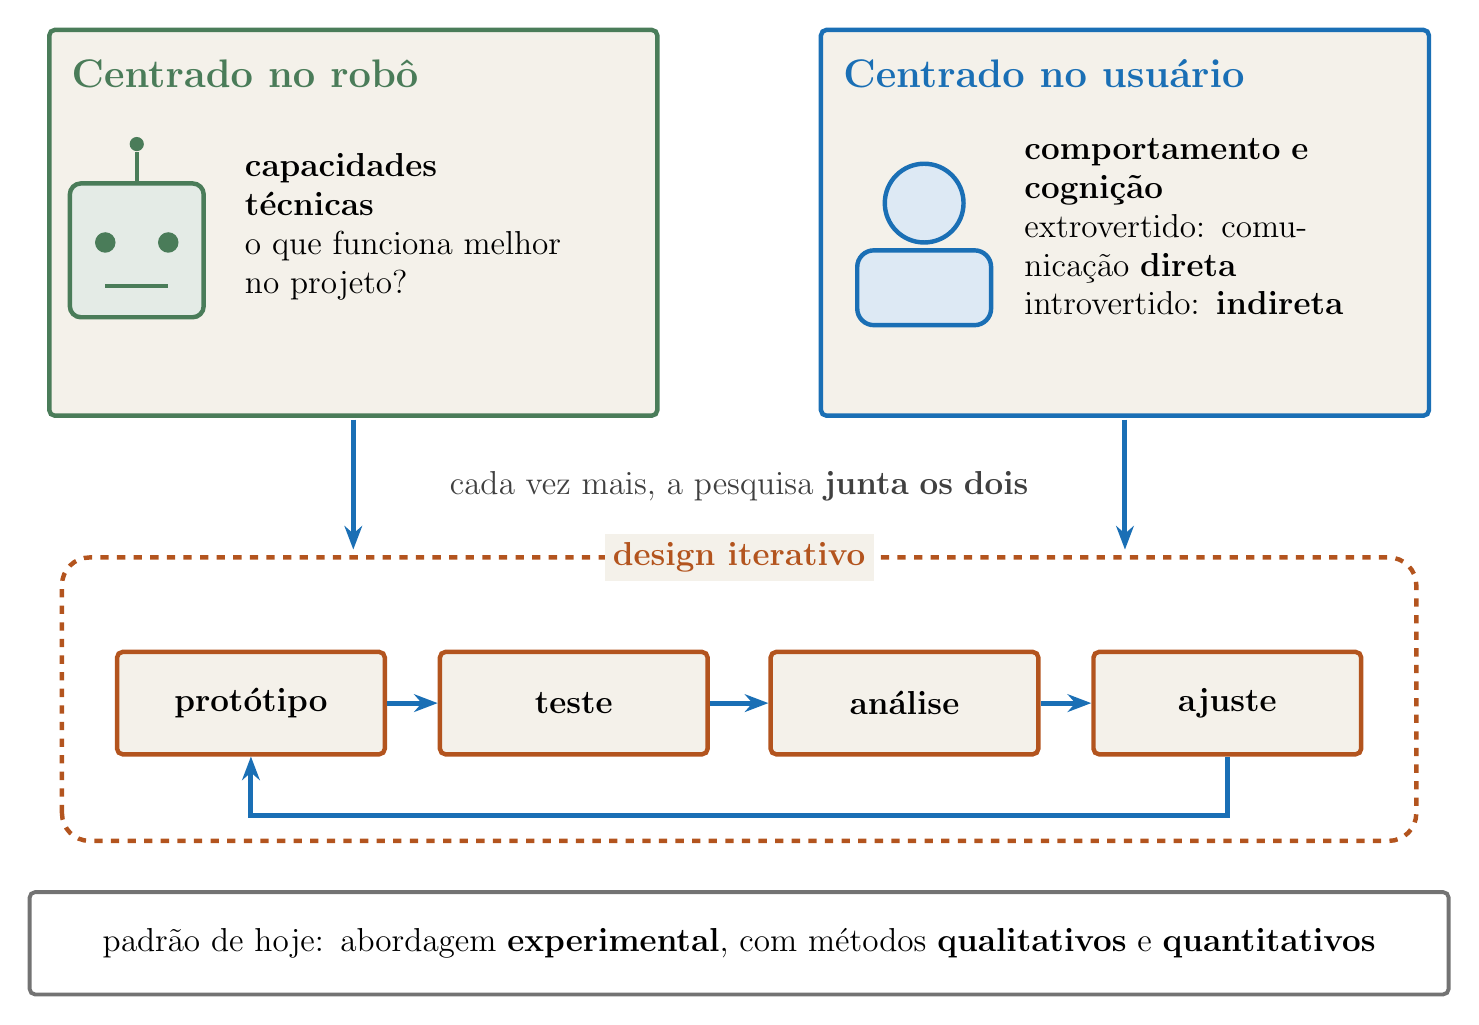
\begin{tikzpicture}[x=1cm,y=1cm]
  \tikzset{card/.style={dbox, text width=7.3cm, minimum height=4.9cm, font=\large, line width=1.6pt, align=left}}
  % ---------- centrado no robô ----------
  \node[card, draw=dgreen] (cr) at (4.6,8.4) {};
  \node[font=\Large\bfseries, dgreen, anchor=west] at (0.9,10.3) {Centrado no robô};
  % ícone: robô
  \draw[dgreen, fill=dgreen!15, line width=1.6pt, rounded corners=4pt] (1.0,7.2) rectangle (2.7,8.9);
  \fill[dgreen] (1.45,8.15) circle (0.13); \fill[dgreen] (2.25,8.15) circle (0.13);
  \draw[dgreen, line width=1.4pt] (1.45,7.6) -- (2.25,7.6);
  \draw[dgreen, line width=1.4pt] (1.85,8.9) -- (1.85,9.3); \fill[dgreen] (1.85,9.4) circle (0.09);
  \node[font=\large, text width=4.1cm, align=left, anchor=west] at (3.1,8.35) {\textbf{capacidades técnicas}\\ o que funciona melhor no projeto?};
  % ---------- centrado no usuário ----------
  \node[card, draw=dblue] (cu) at (14.4,8.4) {};
  \node[font=\Large\bfseries, dblue, anchor=west] at (10.7,10.3) {Centrado no usuário};
  % ícone: pessoa
  \draw[dblue, fill=dblue!15, line width=1.6pt] (11.85,8.65) circle (0.5);
  \draw[dblue, fill=dblue!15, line width=1.6pt, rounded corners=6pt] (11.0,7.1) rectangle (12.7,8.05);
  \node[font=\large, text width=4.1cm, align=left, anchor=west] at (13.0,8.35) {\textbf{comportamento e cognição}\\ extrovertido: comunicação \textbf{direta}\\ introvertido: \textbf{indireta}};
  % ---------- design iterativo ----------
  \draw[dorange, dashed, line width=1.6pt, rounded corners=10pt] (0.9,0.55) rectangle (18.1,4.15);
  \node[font=\large\bfseries, dorange, fill=dcream, inner sep=3pt] at (9.5,4.15) {design iterativo};
  \draw[dtrans, line width=1.8pt, -{Stealth[length=3mm]}] (4.6,5.9) -- (4.6,4.25);
  \draw[dtrans, line width=1.8pt, -{Stealth[length=3mm]}] (14.4,5.9) -- (14.4,4.25);
  \node[font=\large, black!75, text width=8.4cm, align=center] at (9.5,5.05) {cada vez mais, a pesquisa \textbf{junta os dois}};
  \tikzset{e/.style={dbox, draw=dorange, line width=1.6pt, minimum width=3.4cm, minimum height=1.3cm, font=\large\bfseries}}
  \node[e] (p) at (3.3,2.3) {protótipo};
  \node[e] (t) at (7.4,2.3) {teste};
  \node[e] (a) at (11.6,2.3) {análise};
  \node[e] (j) at (15.7,2.3) {ajuste};
  \draw[dtrans, line width=1.8pt, -{Stealth[length=3mm]}] (p.east) -- (t.west);
  \draw[dtrans, line width=1.8pt, -{Stealth[length=3mm]}] (t.east) -- (a.west);
  \draw[dtrans, line width=1.8pt, -{Stealth[length=3mm]}] (a.east) -- (j.west);
  \draw[dtrans, line width=1.8pt, -{Stealth[length=3mm]}] (j.south) -- ++(0,-0.75) -| (p.south);
  % ---------- faixa final ----------
  \node[dbox, draw=black!55, fill=white, line width=1.4pt, text width=17.6cm, minimum height=1.3cm, font=\large, align=center] at (9.5,-0.75) {padrão de hoje: abordagem \textbf{experimental}, com métodos \textbf{qualitativos} e \textbf{quantitativos}};
\end{tikzpicture}
\end{document}
